
%(BEGIN_QUESTION)
% Copyright 2015, Tony R. Kuphaldt, released under the Creative Commons Attribution License (v 1.0)
% This means you may do almost anything with this work of mine, so long as you give me proper credit

\noindent

\vskip 5pt



\vskip 5pt
\begin{center}
\textbf{Styresystemer -- Nivå 2 }
\vskip 5pt 
\textbf{Arbidsoppdrag på Stasjon 3/4}
\vskip 5pt 
\textbf{Programmering av reguleringsstasjon}
\end{center}

\vskip 10pt 
\textbf{Introduksjon}

\vskip 5pt 
Dette oppdraget skal du programmere en Gand reguleringsstasjon. Du kan velge mellom stasjon03 og stajson04. Du skal følge samme fremgangmåte som i programmeringen av nivå 1 oppdraget. 

Programmet diss skal gjøre det mulig å regulere nivået i tanken og strømningen ut av tanken. 
\href{https://rfka-my.sharepoint.com/:u:/g/personal/fred-olav_mosdal_skole_rogfk_no/EewzybzUnq5PscHy_uJUvUMB3ufsOB417mgUkhGlC8yQrg?e=rPkbpf}{Eksempel program med PID i codesys}

\vskip 5pt 

\vskip 5pt 

$$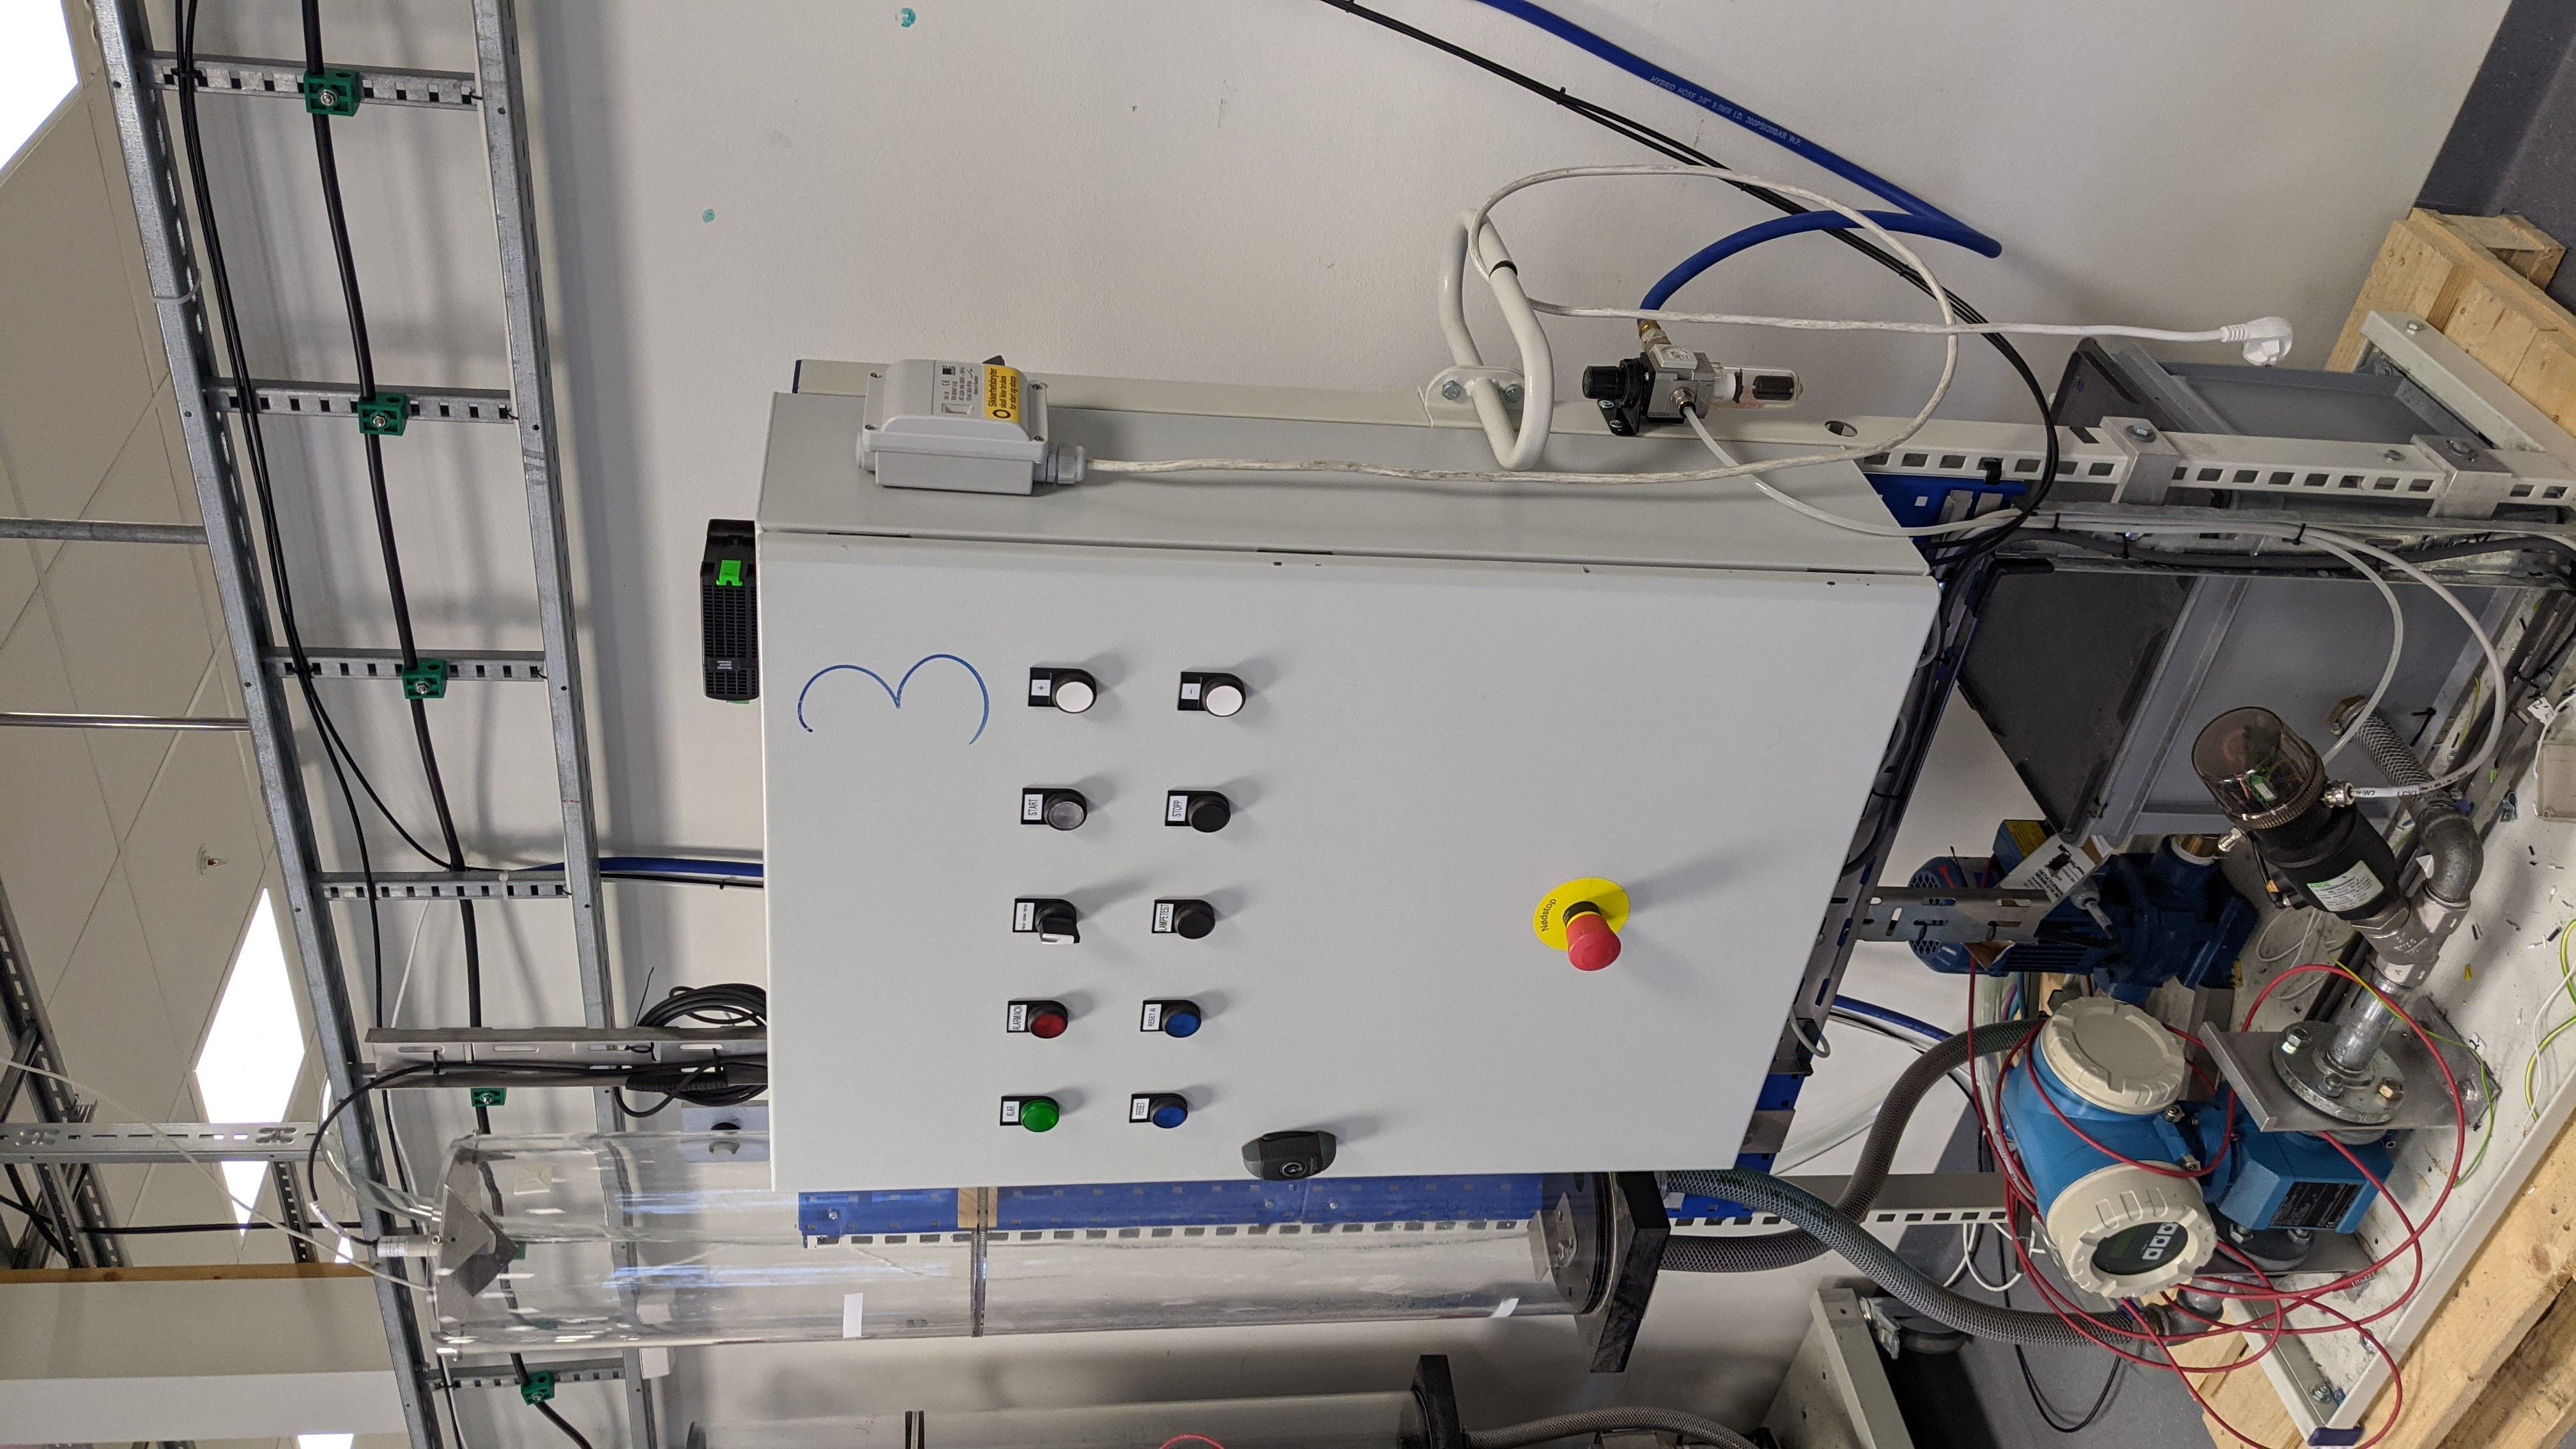
\includegraphics[width=10.5cm,angle=-90]{stasjon03x01.jpg},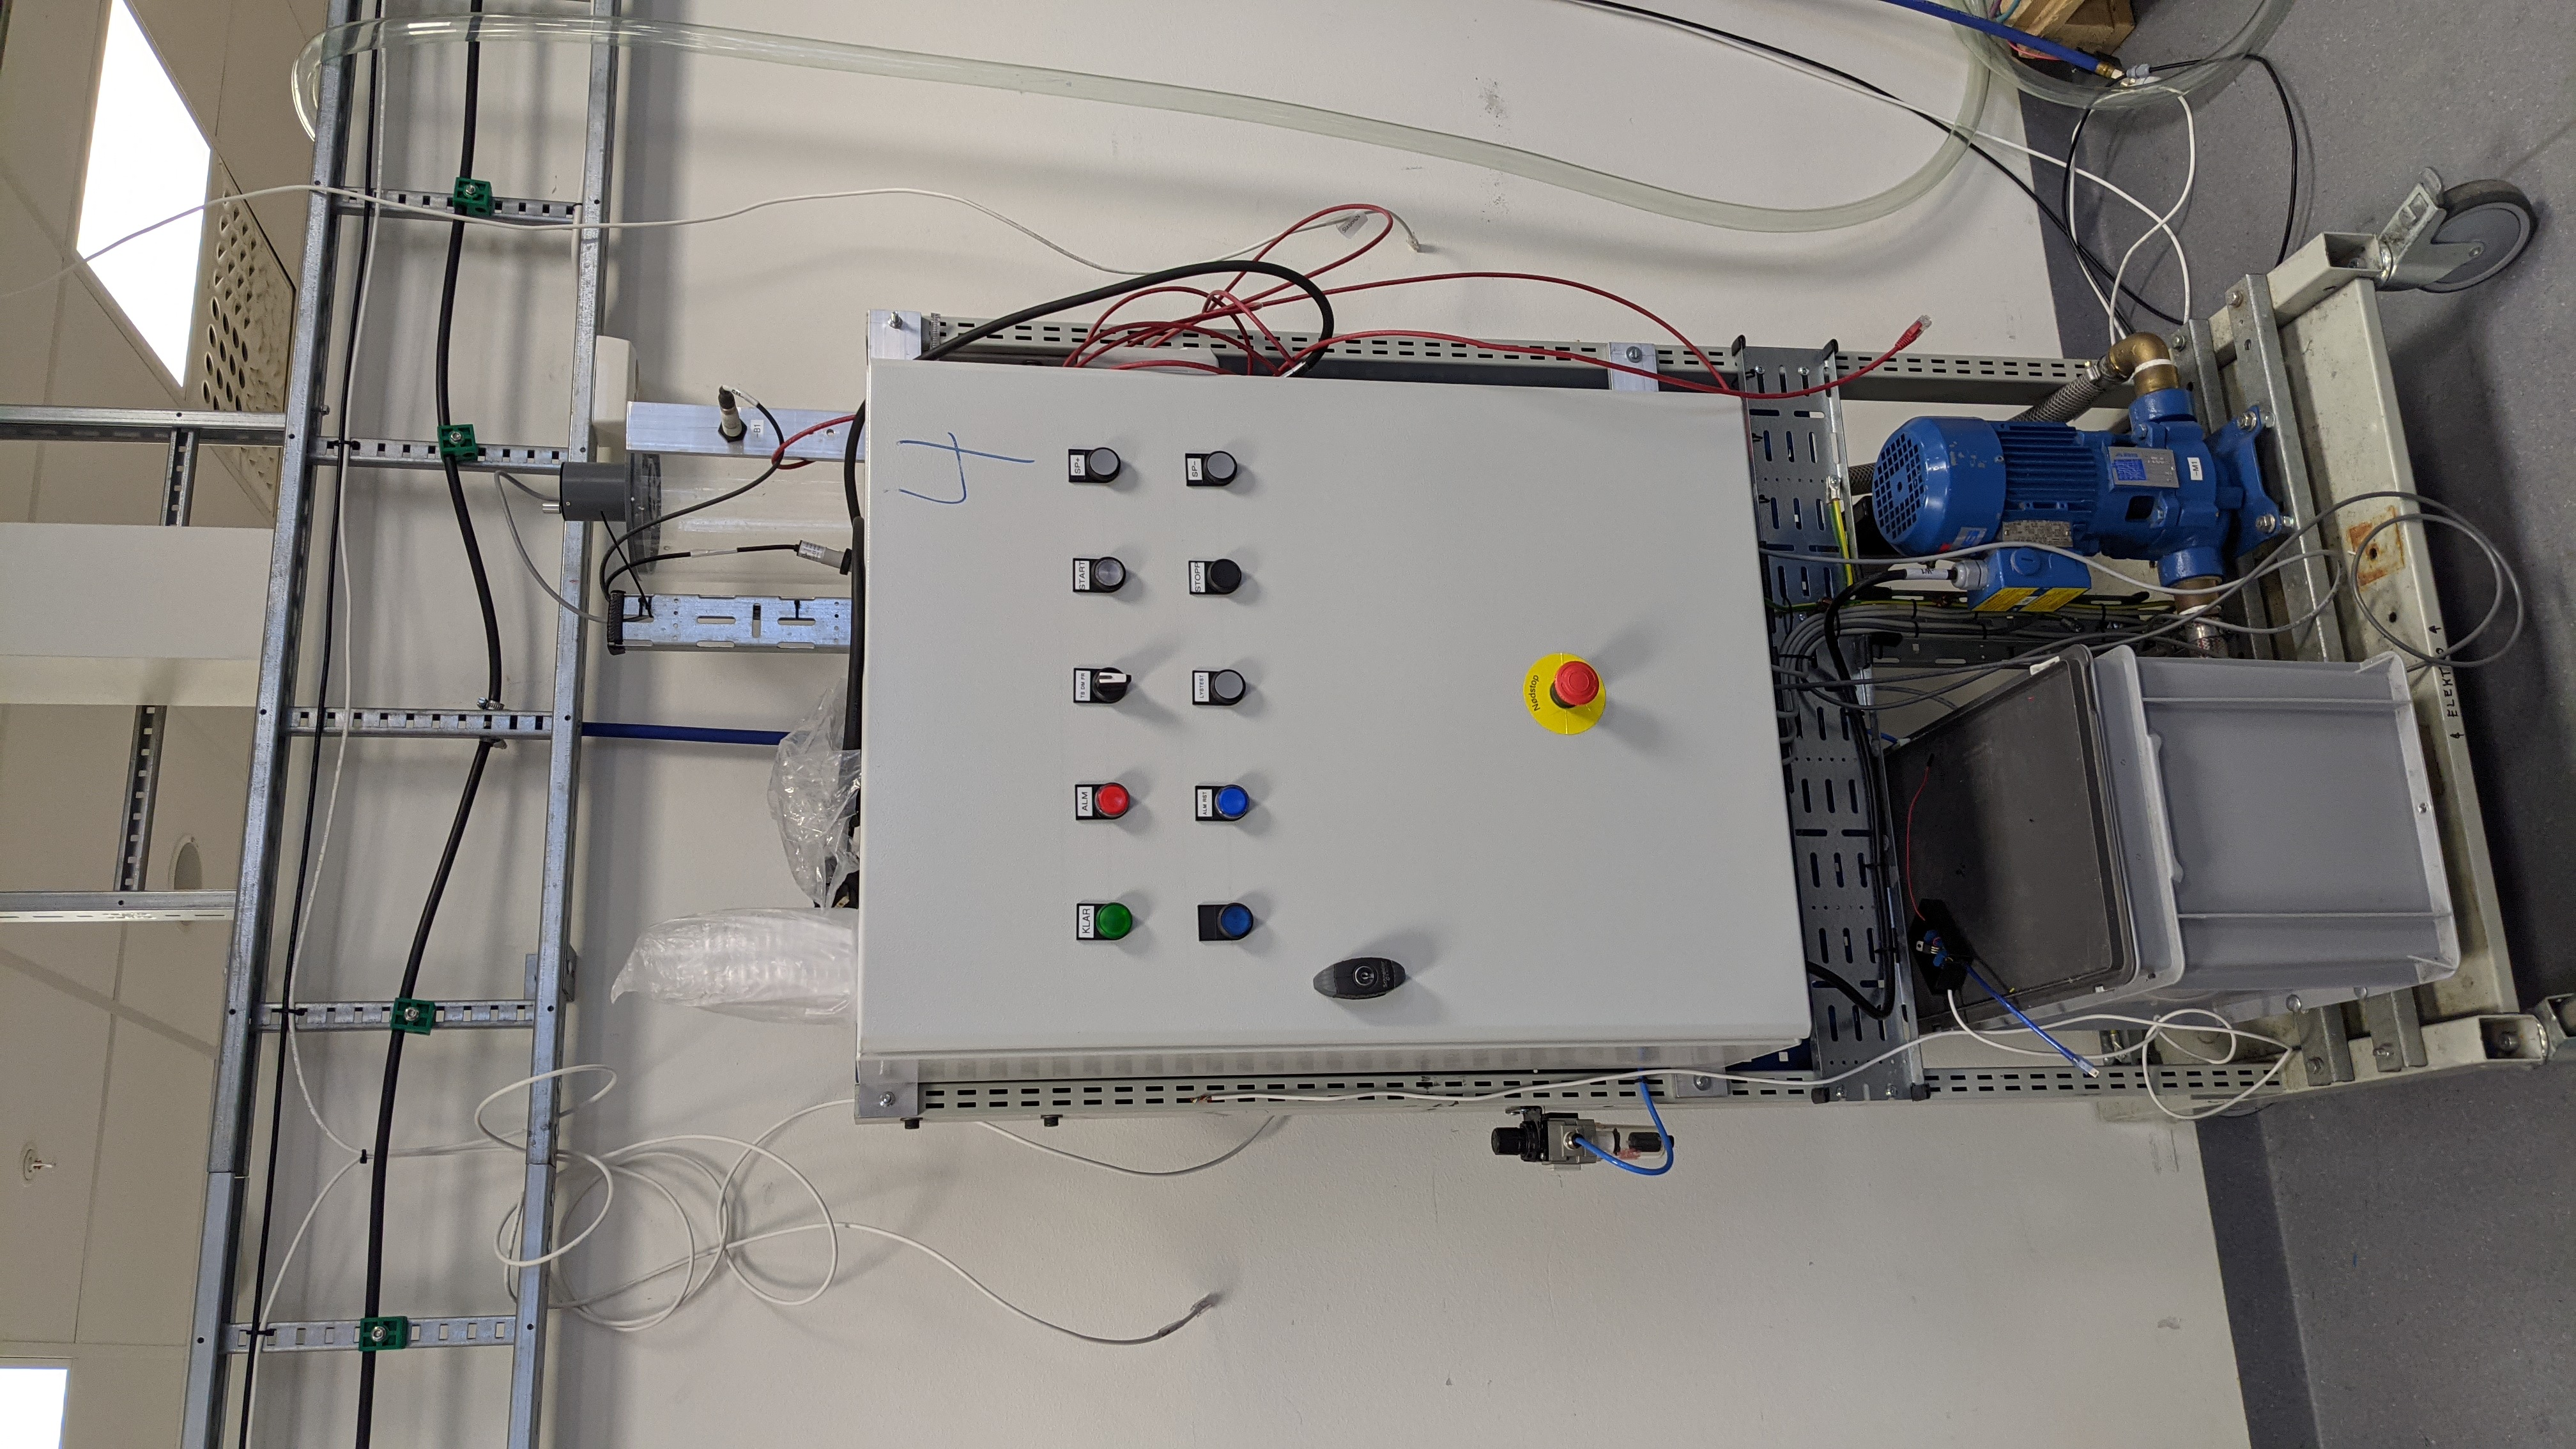
\includegraphics[width=10.5cm,angle=-90]{stasjon04x01.jpg}$$

\vskip 10pt 
\textbf{Teorioppgaver}
Leseoppgave:

\vskip 5pt 
\url {https://autofaget.no/closedloop/node2.html}
\vskip 5pt 
Oppgavehefte:
\vskip 5pt 
https://autofaget.no/pdfs/Regulering.pdf
\vskip 5pt 

\vskip 10pt 
\textbf{Planlegging}


\vskip 10pt 
\textbf{Gjennomføring}

\vskip 10pt 
\textbf{Dokumentasjon}

%$$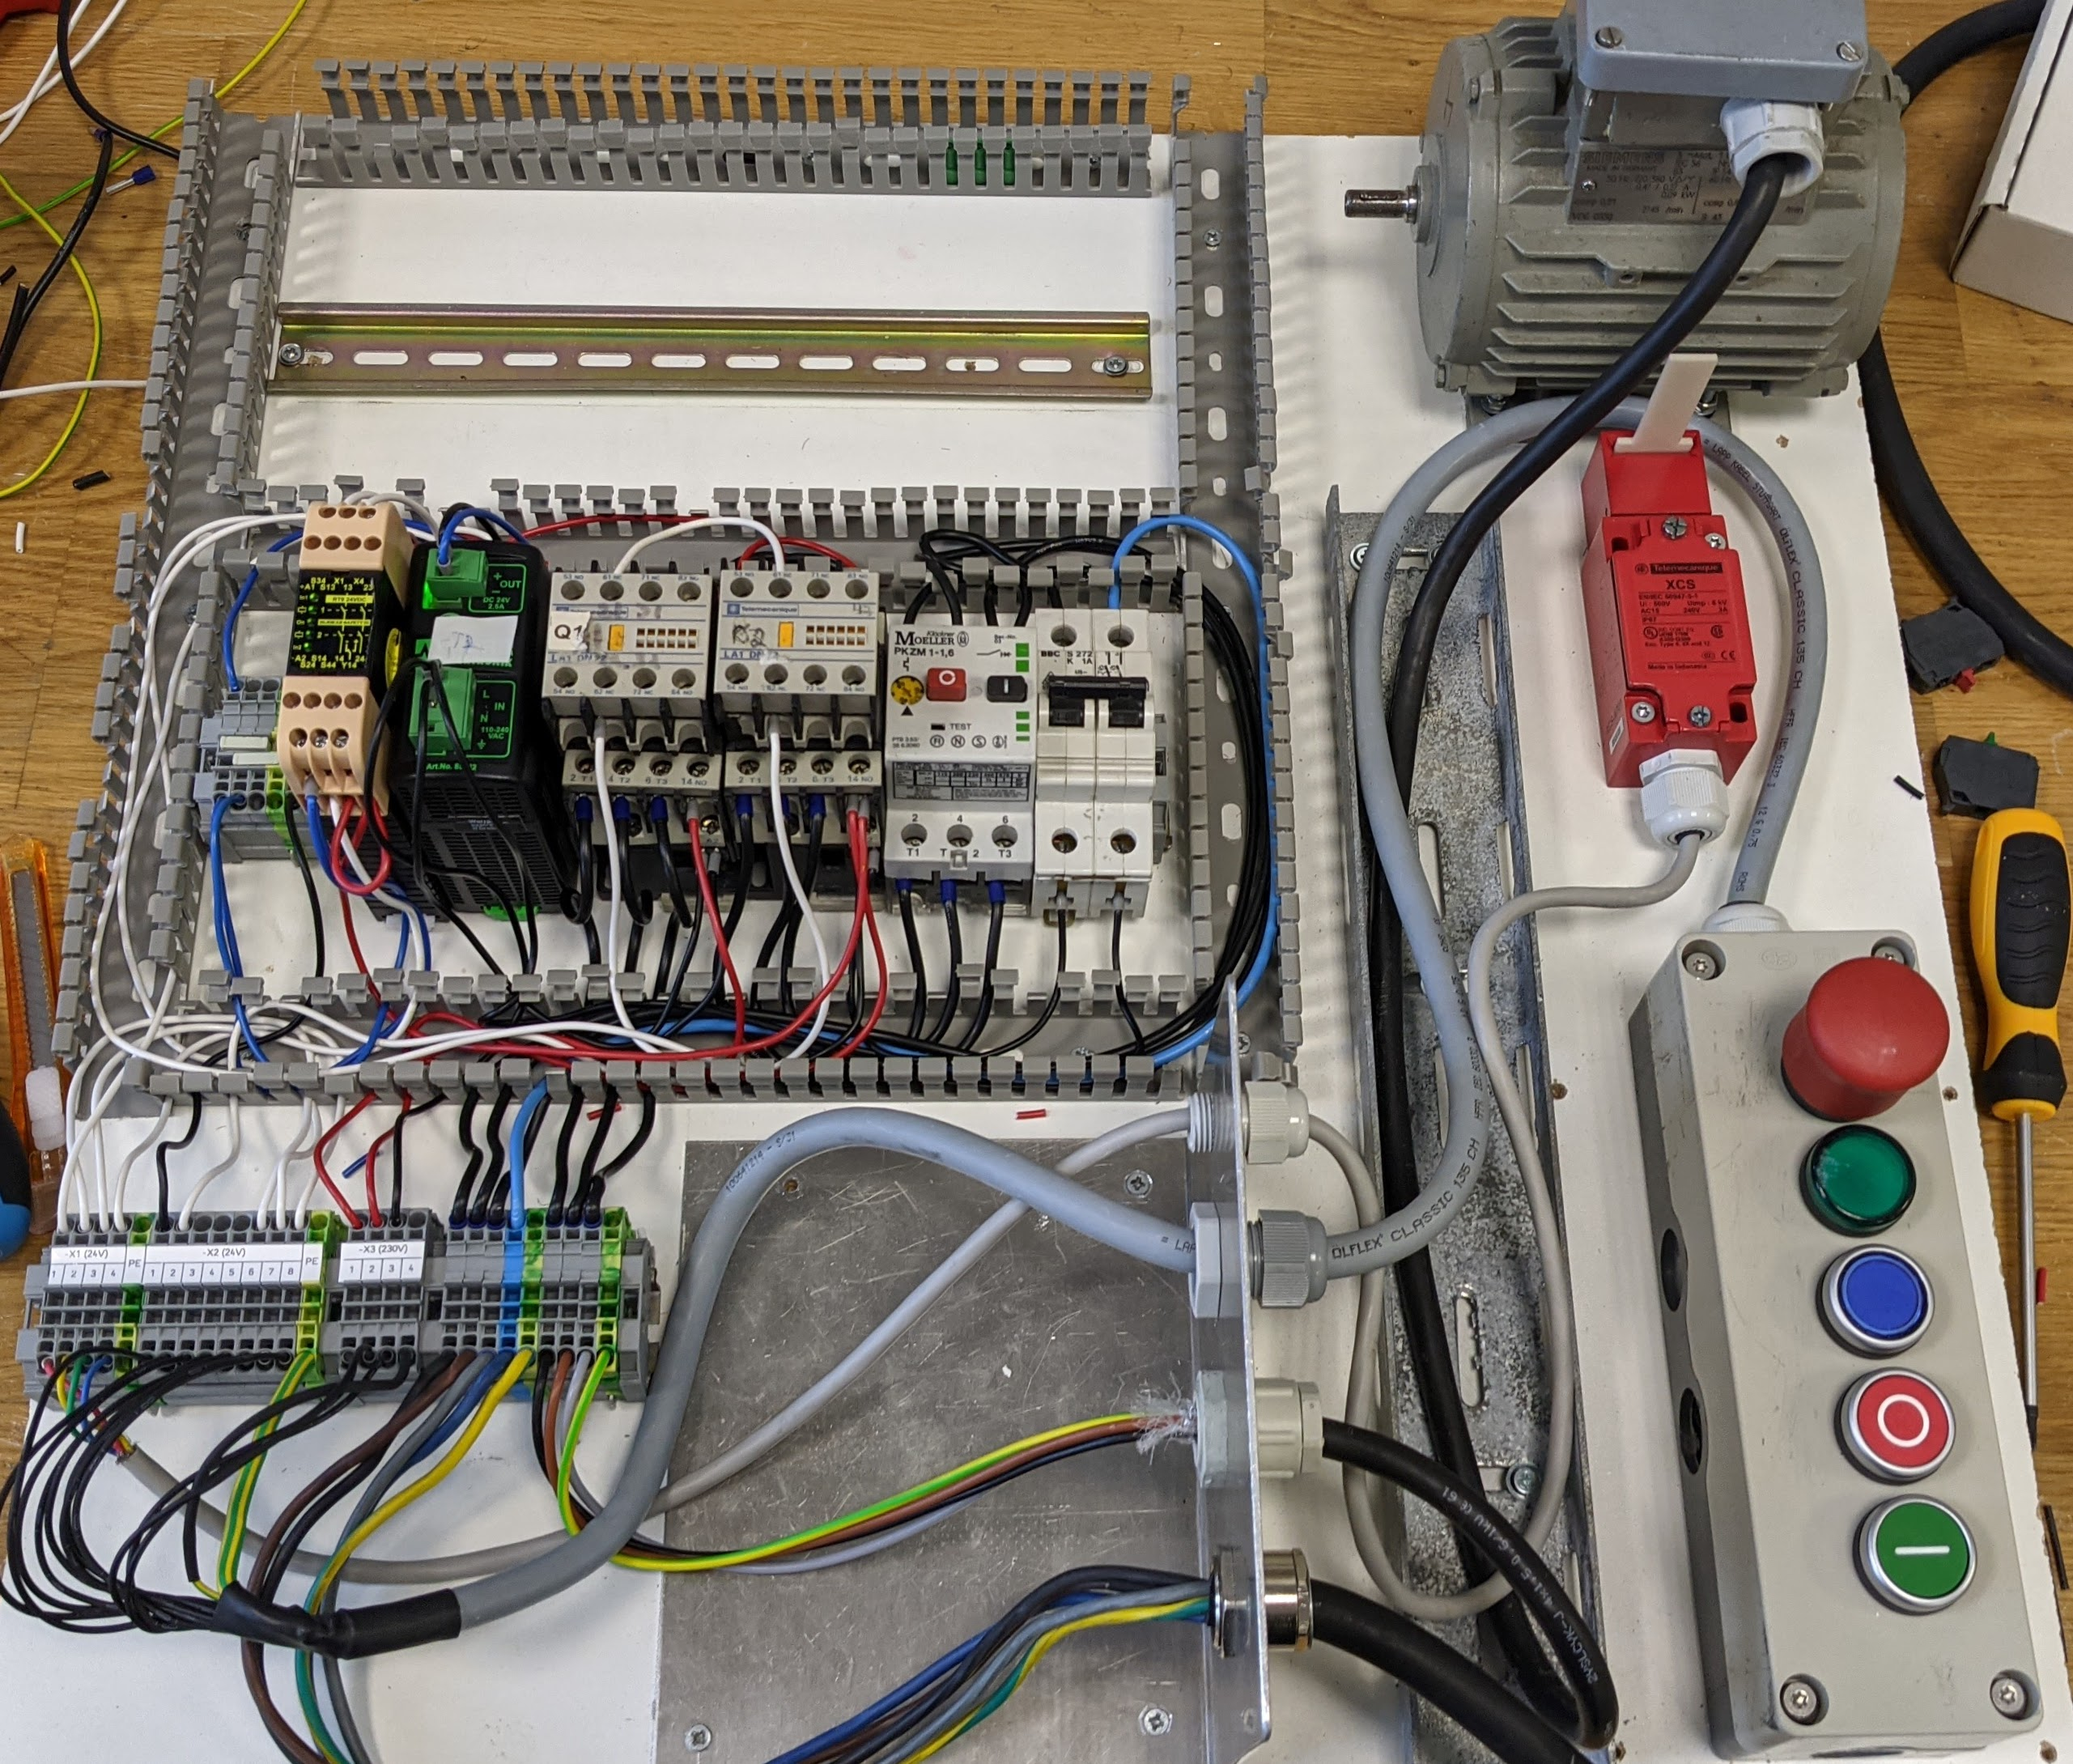
\includegraphics[width=13cm]{i04821x01.jpg}$$\\
















\underbar{file i04824}
\vfil \eject
%(END_QUESTION)





%(BEGIN_ANSWER)


%(END_ANSWER)





%(BEGIN_NOTES)


%INDEX% Arbeisdoppdrag, Styresystemer, Nivå 2, Stasjon03/04, Programmering av reguleringsstasjon

%(END_NOTES)


